\documentclass[12pt]{article}  
\usepackage{pgf}
\usepackage{tikz}
\usetikzlibrary{automata}
\usepackage[latin1]{inputenc}
\usepackage{latexsym,amsmath}
\voffset=-.8cm
\hoffset=-2cm
\setlength{\textheight}{22.60cm}
\setlength{\textwidth}{14.00cm}
\pagestyle{myheadings}
\newtheorem{q} {Q}
\newcommand{\beq}{\begin{q}\hskip-.2cm)}
\newcommand{\eeq}{\end{q}\newpage}
\newtheorem{dfntn}{Definition}
\newcommand{\df}{\displaystyle\frac}
\markright {Dr. Petrescu CCP MATH263 Homework 4}
\begin{document}
{\bf Practice Exam 3  Discrete Mathematics II} \vskip0.2cm
{\bf Name}: \rule{8cm}{.01cm} \hspace*{0.2cm} {\bf  Due Date}: \underline{04/08} 
%%%questions
\beq  (i) How many nonisomorphic non rooted  trees are there with 4 vertices ? \\  (ii) How many nonisomorphic rooted trees are there with 4 vertices?  \\(iii) How many nonisomorphic  {\bf non rooted}  trees are there with 5 vertices  \eeq
\beq  a. How many edges does a tree with 10,000 vertices have? \par b.  How many vertices does a full 5-ary tree with 100 internal vertices have? \par c. How many edges does a full binary tree with 1000 internal vertices have? \par d. How many leaves does a full 3-ary tree with 100 vertices have?\eeq
\beq Suppose that the address of the vertex $v$ in the ordered rooted tree $T$ is 3.4.5.2.4. \\ a) At what level is $v$? \\ b) What is the address of the parent of $v$?\\ c) What is the least number of siblings $v$ can have? \\ d) What is the smallest possible number of vertices in $T$ if $v$ has this address?\eeq
\beq Use depth- first search to find a spanning tree of each of these graphs. \\ a) $W_6$ , starting at the vertex of degree 6\hskip 2cm b) $K_5$ \\ c) $K_{3,4}$, starting at a vertex of degree 3 \hskip2.1cm d) $Q_3$\eeq
\beq Prove Kruskal's Theorem \eeq
\beq Use Prim-Jarnik's or Kruskal's algorithm to find, step by step, the minimal spanning tree from the graph below. State what method you are using.\vskip1cm
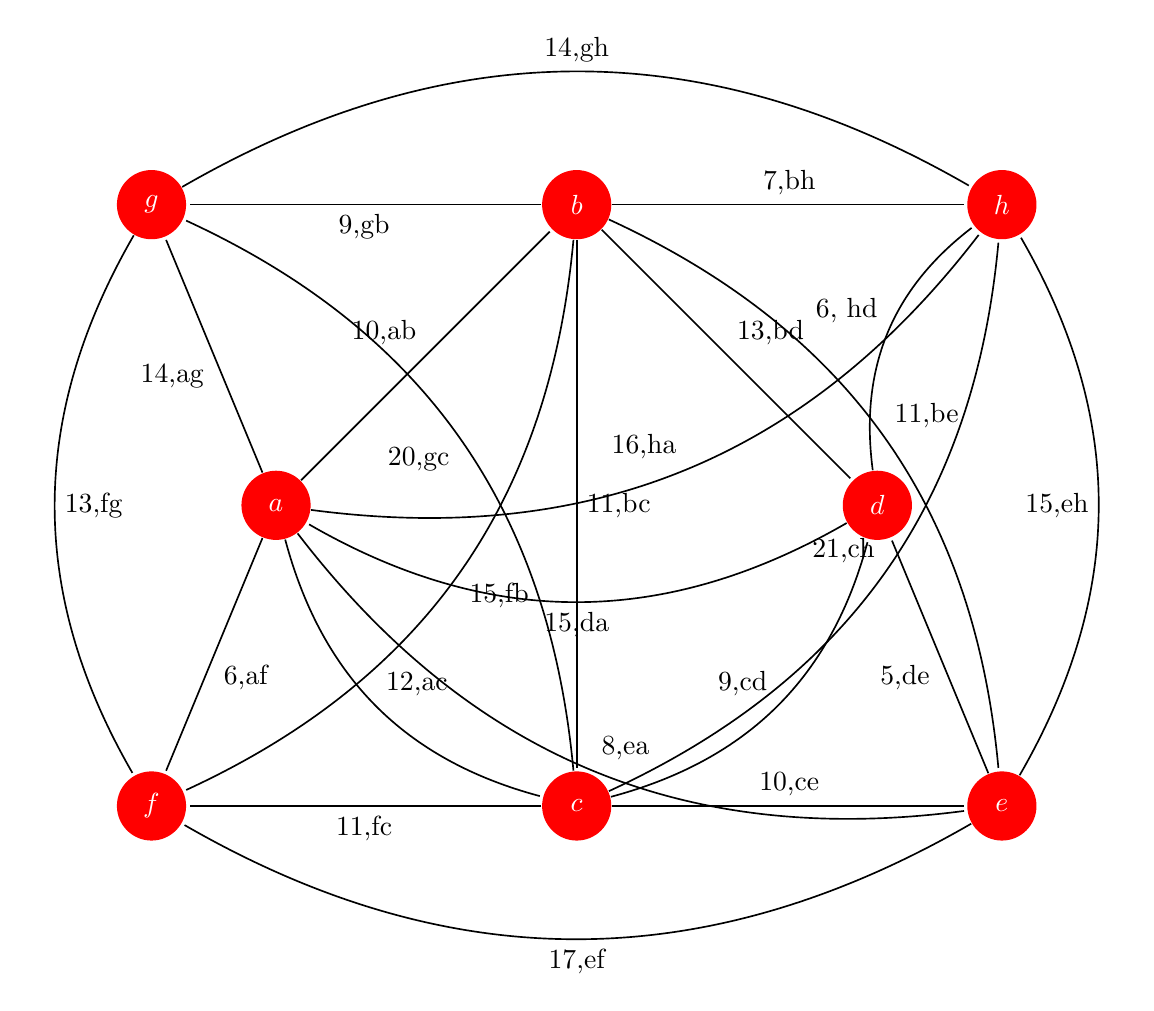
\begin{tikzpicture}[- ,shorten   >=1pt, auto, node distance=5.4cm, semithick]  %, >=stealth', 
  \tikzstyle{every state}=[fill=red,draw=none,text=white]
  \node[state] 	     (A)                             {$a$}; %initial,
  \node[state]         (B) [above right of=A] {$b$};
  \node[state]         (C) [below right of=A] {$c$};
  \node[state]         (D) [below right of=B] {$d$};
  \node[state]         (E) [right of= C]          {$e$};	
  \node[state]         (F) [ left of=C]          {$f$};
  \node[state]         (G) [left of=B]          {$g$};
  \node[state]         (H) [right of=B]          {$h$};
  \path (A) edge                 node  [auto] {10,ab} (B)
            	edge                [bend right]  node [auto] {12,ac} (C)
	           edge                node  [auto] {14,ag} (G)
            	edge               [bend right] node  [auto] {16,ha} (H)
            	edge              node [auto] {6,af} (F)
            	edge              [bend right] node [auto] {8,ea} (E)

         (B)   edge          node  [auto] {11,bc} (C)
                 edge           node  [auto] {13,bd} (D)
                 edge          [bend left]           node  [auto]  {15,fb} (F)
                 edge            node   [auto] {9,gb} (G)
                 edge         [bend left]      node [auto] {11,be} (E)
                 edge              node [auto] {7,bh} (H)
                 
            (C) edge        [bend right]    node [auto] {9,cd} (D)
                  edge               node [auto] {10,ce} (E)
                  edge              node [auto] {11,fc} (F)
                  edge        [bend right]       node [auto] {21,ch} (H)
                  edge        [bend right]       node  [auto]{20,gc} (G)

 		(E)   edge      [bend right]        node  [auto] {15,eh} (H)
               	         edge      [bend left]           node [auto] {17,ef } (F)
		        edge               		         node [auto] {5,de} (D)
			
		(G)   edge      [bend right]           node [auto] {13,fg} (F)
 		         edge      [bend left]              node [auto]  {14,gh} (H)
			
			
       		 (D)   edge       [bend left]         node [auto] {15,da} (A)
       			edge          [bend left]        node [auto] {6, hd} (H);

\end{tikzpicture}\eeq
\beq Describe the tree produced by breadth-first search and depth-first search for the n-cube graph $Q_n$, where n is a positive integer.\eeq
\begin{q} \label{q:questao0} Build a binary search tree for the words: {\em oenology, phrenology, campanology, ornithology, ichthyology, limnology, alchemy,} and {\em astrology} using alphabetical order.\end{q}\newpage
\begin{q}  For the tree in question \ref{q:questao0}  determine the order in which a inorder traversal visits the vertices of the given ordered rooted tree.                \end{q}\newpage
\begin{q}  For the tree in question \ref{q:questao0}  determine the order in which a postorder traversal visits the vertices of the given ordered rooted tree.             \end{q}\newpage
\begin{q}  How many nonisomorphic unrooted trees are there with six vertices? \end{q}\newpage
\begin{q} How many nonisomorphic rooted trees are there with six vertices ?\end{q}\newpage

%%%questions
\end{document}